\documentclass[12pt,a4paper]{article}
\usepackage[T1]{fontenc}
\usepackage[polish]{babel}
\usepackage[utf8]{inputenc}
\usepackage{lmodern}
\usepackage{graphicx}
\usepackage{wrapfig}
\selectlanguage{polish}


\author{
  Maciej Buczyński\qquad \texttt{kadlubken5@gmail.com}
  \and
  Tomasz Szypuła\qquad \texttt{tszypula@gmail.com}
}
\title{Model Isinga na regularnych grafach przypadkowych}

\begin{document}
\maketitle
\section{Cel ćwiczenia}
Celem ćwiczenia było zapoznanie się z symulacją modelu Isinga na regularnych grafach przypadkowych.

\section{Wstęp teoretyczny}
\subsection{Regularny graf przypadkowy}
Obiekty w układzie zostały połączone w tzw. regularny graf przypadkowy, gdzie obiekty są węzłami grafu, a krawędzie symbolizują połączenia. Zgodnie z definicją takiego grafu, każdy węzeł ma taką samą liczbę krawędzi, które rozmieszczone są losowo.

\subsection{Model Isinga}
Model Isinga opisuje układy, gdzie obiekty mają do wyboru jeden z dwóch różnych stanów. Obiekty te mogą następnie oddziaływać ze sobą, prowadząc do ewolucji czasowej(iteracyjnej) układu. W naszym przypadku stanami były spiny +1 i -1.

Energię dla pojedynczego spinu w modelu Isinga określa wzór:
$$ E_{i}=-s_{i}\sum_{j}s_{j}J_{ij}$$
Gdzie $s_{i}$- i-ty spin, $J_{ij}$- stała oddziaływania między spinami $i$ oraz $j$(w naszym przypadku równa 1- oddziaływanie ferromagnetyczne), a sumowanie odbywa się po wszystkich sąsiadach $s_{i}$
 
\section{Metoda symulacji oraz temperatura krytyczna}
W celu symulacji ewolucji czasowej układu posłużyliśmy się algorytmem Metropolis:
\begin{itemize}
\item Wybranie losowego spinu $i$
\item Kalkulacja różnicy energii w przypadku zmiany spinu
\item Jeśli energia zmaleje, zmiana spinu na przeciwny. Jeśli nie, zmiana spinu jedynie z pewnym prawdopodobieństwem $e^{\frac{-\Delta E}{k_{B}T}}$
\end{itemize}

W czasie dążącym do nieskończoności układ z $T=0$ ulegnie samoistnej magnetyzacji. Jednak dla pewnej wartości $T_c$ szumy termiczne będą tak duże, że układ nie będzie wykazywał magnetyzacji, tzn. M=0. Wzór teoretyczny dla temperatury krytycznej:
$$ T_{c}=\frac{2}{ln(\frac{k}{k-2})} $$
Gdzie $k$- stopień węzła(liczba sąsiadów)

\section{Wyniki}
\subsection{Ewolucja czasowa}
Tutaj walniemy time spectrum
\subsection{Wykresy temperaturowe}
Tutaj walniemy trochę wykresów temperaturowych

\paragraph{}
Na wykresach \ref{fig:TcOd1/N.1} oraz \ref{fig:TcOd1/N.2} wyraźnie widać, że wartość temperatury krytycznej bardzo szybko zbiega do teoretycznej wartości oczekiwanej. Na przykład dla grafu o stopniu węzłów równym 5, teoretyczna temperatura krytyczna wynosi około $T_{c} = 3.9152$ , już dla liczby węzłów mniejszej od $10^3$ (około 650), błąd wynosi mniej niż $2\%$.

\paragraph{}
Wykresy \ref{fig:LnTcOd1/N.1} oraz \ref{fig:LnTcOd1/N.2} powstały po zlogarytmowaniu poprzednich wykresów. Na wykresach \ref{fig:TcOd1/N.1} oraz \ref{fig:TcOd1/N.2} było widać bardzo szybkie zbieganie temperatury krytycznej, która potencjalnie mogła mieć charakter logarytmiczny. Stąd po zlogarytmowaniu chcieliśmy zobaczyć czy dane rzeczywiście będą układać się w linię prostą.

\paragraph{}
Wykres \ref{fig:TcOdK} podsumowuje poprawne, zgodne z oczekiwaniami, zachowanie się zmiany temperatury krytycznej od stopnia węzłów, dla ustalonej liczby węzłów (w tym przypadku dla około $15*10^3$). We wszystkich przypadkach już dla liczby węzłów mniejszych  od stu tysięcy, błąd wynosi dużo mniej niż ułamki procenta. Dla przykładu dla liczby węzłów około $N = 40000$ oraz stopnia węzłów $K=5$ błąd jest rzędu $10^{-6}\%$.

\begin{figure}
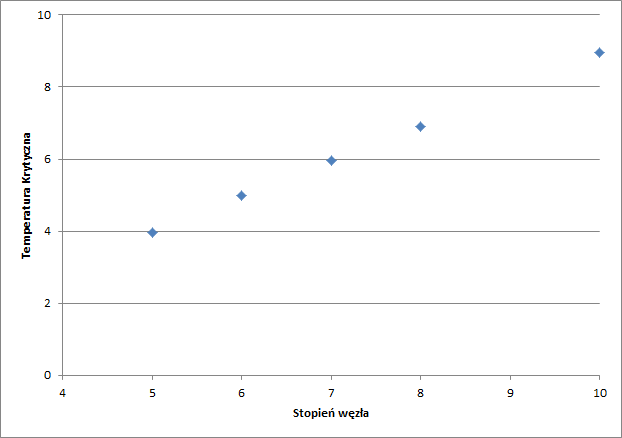
\includegraphics[width=\textwidth]{TodK.png}
\caption{Temperatura krytyczna zmierzona dla różnego stopnia węzła przy stałej liczbie węzłów}
\label{fig:TcOdK}
\end{figure}

\begin{figure}
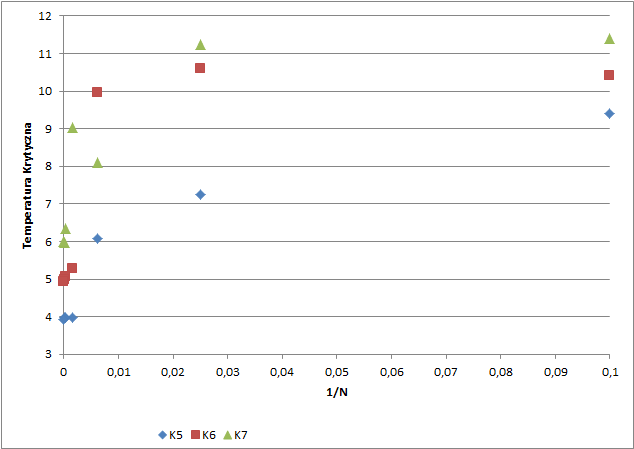
\includegraphics[width=\textwidth]{K5K6K7.png}
\caption{Temperatura krytyczna w zależności od $\frac{1}{N}$, dla różnych stopni węzła}
\label{fig:TcOd1/N.1}
\end{figure}

\begin{figure}
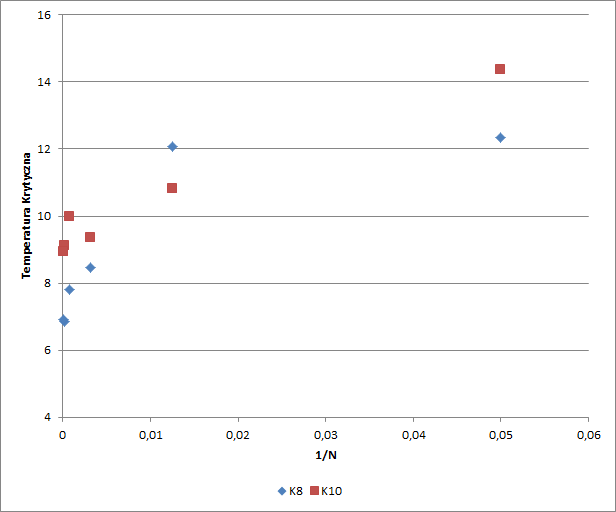
\includegraphics[width=\textwidth]{K8K10.png}
\caption{Temperatura krytyczna w zależności od $\frac{1}{N}$, dla różnych stopni węzła}
\label{fig:TcOd1/N.2}
\end{figure}

\begin{figure}
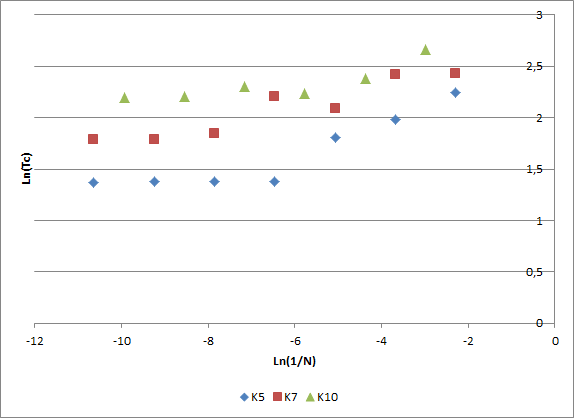
\includegraphics[width=\textwidth]{LNK5K7K10.png}
\caption{Logarytm naturalny z Temperatura krytyczna w zależności od $\ln(\frac{1}{N})$, dla różnych stopni węzła.}
\label{fig:LnTcOd1/N.1}
\end{figure}

\begin{figure}
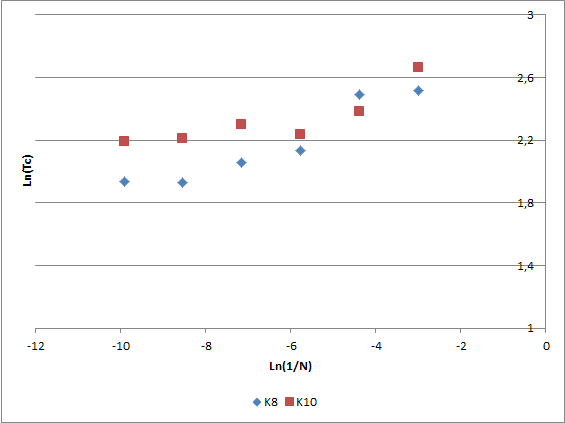
\includegraphics[width=\textwidth]{LNK8K10.png}
\caption{Logarytm naturalny z Temperatura krytyczna w zależności od $\ln(\frac{1}{N})$, dla różnych stopni węzła.}
\label{fig:LnTcOd1/N.2}
\end{figure}

\subsection{Inne zależności}
Tutaj całą resztę

\section{Wnioski}
\begin{itemize}
\item Bla bla bla, wszystko wyszło
\end{itemize}
\end{document}